% ------------------------------------------------------------------------
% -*-TeX-*- -*-Hard-*- Smart Wrapping
% ------------------------------------------------------------------------
\def\baselinestretch{1}

\chapter{Development}
\label{chapter:Development}

\def\baselinestretch{1.66}


%%% ----------------------------------------------------------------------

This chapter chronicles the development of the application, as well as testing of each individual element of the project as it is developed, in order to further refine it. This testing should not be confused with the testing section (chapter \ref{chapter:Testing}), which is larger scale testing of interactivity between system components, and of the system as a whole.

%%% ----------------------------------------------------------------------
\goodbreak

\section{Investigations}
\label{sec:Investigations}
This section chronicals experimentation undertaken to develop skills and basic \textcolor{red}{frameworks} using technologies identified as being useful to the project.

At the end of each of these sections, a series of aspects which will be included in the main project are outlined.

\subsection{Java and JSON}
\label{subSec:Java and JSON}

\subsection{Three.js}
\label{subSec:Three.js}
This is a log and index of experiments using Three.js, particularly with a mind to integrating the technology into the project; Blender, JSON etc. The project is divided into a series of labs, which chronicle the changes made by session.

\subsubsection{Lab 1: 28/12/2015: First Three.js experiment}
\label{subSubSec:ThreeJSExperiments:Lab1}
his is a very simple HTML file displaying a rotating cube. It is a excercise in the basics of using Three.js for WebGL.

\subsubsection{Lab 2: 30/12/2014: .Obj file loader test: Local library access}
\label{subSubSec:ThreeJSExperiments:Lab2}
The first stage of this lab was to reverse engineer JavaScript data found associated with \url{http://threejs.org/examples/webgl_loader_obj.html} \textcolor{red}{[CITE THIS]}, which features use of OBJLoader.js; part of the Three.js library which allows for the importation of .OBJ files for display through JavaScript.

This JavaScript file first copied and tested by changing the .OBJ file link from the one within the Three.js library specified in the demo for a model of a car taken from \url{http://tf3dm.com/3d-models/bmw850/1/obj} \textcolor{red}{[CITE THIS]}, and reskinned with a plain white texture.

\subsubsection{Lab 3: 06/01/2015: .Obj file loader test: Remote library access}
\label{subSubSec:ThreeJSExperiments:Lab3}
A repeat of lab 2, attempting to reference the Three.js library from its location online, rather than locally

Unfortunatly, attempts to access the files as online resources through http://cdnjs.com/libraries/three.js/, my dropbox account and github all failed. As such, the large local three.js library and this project will be relocated as part of the DataCentreModelling project, in order to conserve space.

\subsubsection{Lab 4: 06/01/2015: Object animation tutorial}
\label{subSubSec:ThreeJSExperiments:Lab4}
Following of a tutorial at\url{http://code.tutsplus.com/tutorials/webgl-with-threejs-basics--net-35688} \textcolor{red}{[CITE THIS]} to develop an animated cube object, without the need to import an external .obj file into the project.

\subsubsection{Lab 5: 08/01/2015: Camera animation tutorial modification}
\label{subSubSec:ThreeJSExperiments:Lab5}
Lab 4 is repeated, animating the camera to spin on it's Y axis, rather than the cube object.

\subsubsection{Lab 6: 12/01/2015: TrackballControl.js: A development of the page ``WebGL With Three.js: Basics"} 
\label{subSubSec:ThreeJSExperiments:Lab6}
A modification of \url{http://code.tutsplus.com/tutorials/webgl-with-threejs-basics--net-35688} \textcolor{red}{[CITE THIS]}, exchanging pyramids for cubes.

This experiment is undertaken to explore the potential of TrackballControls.js within the Three.js library

This was tested both on a Windows 7 system, and an Android tablet. The windows testing revealed that clicking and dragging on any part of the page would pan the camera around the scene, and using the mousewheel would zoom the camera into the scene (forward for zooming in, backward for zooming out). The testing on the Android tablet revealed that touching and dragging on the page rotated the camera around the scene, pinching outwards with two fingers zoomed the camera out from the scene, pinching inwards with two fingers zoomed the camera into the scene, and dragging two fingers across the screen moved the camera along an axis relative to the 3D object.

\subsubsection{Lab 7: 12/01/2015: A single lit object viewed by a trackball controlled camera}
\label{subSubSec:ThreeJSExperiments:Lab7}
A development of the work in Lab 4 (and by extention http://code.tutsplus.com/tutorials/webgl-with-threejs-basics--net-35688), producing more of a blank canvas, with the ultimate goal of producing a template JavaScript file (or collection of files) to use in the DataCentreModelling project.

\subsubsection{Lab 8: 14/01/2015: A single lit, animated object viewed by a trackball controlled camera}
\label{subSubSec:ThreeJSExperiments:Lab8}
This features an .obj 3D object file imported into the scene using an OBJLoader class object, coloured with a plain white JPEG file, and illuminated from one side by a red spotlight. The scene is also observed by a camera controlled by a TrackBallConrols class object, allowing free movement, rotation and zooming of the camera relative to the scene.

\subsubsection{Lab 9: 15/01/2015: Lighting experiment}
\label{subSubSec:ThreeJSExperiment:Lab9}
An attempt was made to produce variable colour and three.js spotlights, controlled by HTML buttons linked to embedded JavaScript was made. This failed, and was postponed due to not being essential to the project.

\subsubsection{Lab 10: 21/01/2015: Implementation of three.js voxel painter at ``three.js webgl - interactive - voxel painter"}
\label{subSubSec:ThreeJSExperiments:Lab10}
This is an implementation of source code found at \url{http://threejs.org/examples/webgl_interactive_voxelpainter.html} \textcolor{red}{[CITE THIS PROPERLY]}, which displays a three.js based voxel painting canvas.

This implements the use of "voxels", or volumetric pixels, which are added as coloured cubes to a three dimentional grid plane. This makes an interesting potential basis for the data centre modelling application: This grid-plane system could be used, with the voxels replaced by 3D objects representing items being added to the data centre floor.

\subsubsection{Lab 11: 24/01/2015: Combination of three.js voxel painter with TrackballCamera.js}
\label{subSubSec:ThreeJSExperiments:Lab11}
This experiment brings together two different projects, Lab 7 (and by extention \url{http://threejs.org/examples/webgl_interactive_voxelpainter.html} \textcolor{red}{[CITE THIS]}) and \textcolor{red}{three.js - interactive - voxel painter [CITE THIS PROPERLY- IT WAS CITED IN LAB 10]}, producing a 3D voxel painter, using a three.js rollover mesh, a rollover helper when the cursor passes over the mesh, and allowing a black 3D cube to be placed wherever the rollover helper is when the mouse is clicked, and for the camera to be moved around the scene by the by clicking and dragging the cursor, making for intuitive control of the voxel painter, including camera relocation.

\subsubsection{Lab 12: 04/03/2015: Inclusion of 3D objects generated from JSON files into Lab-11}
\label{subSubSec:ThreeJSExperiments:Lab12}
This is a development of lab-11, replacing the Three.js BoxGeometry cubes placed on the grid with a 3D object imported from an external file, as was the case with lab-8 and before.

Unlike lab-8, the file used to generate the 3D cones placed by clicking on the grid is a JSON file rather than an .obj file; this is because it was found to be difficult to sucessfully cast the three.js .obj file loader class object, OBJLoader, into the framework that already existed in lab-11, where as the class which interprets JSON files as 3D objects, JSONLoader, is possible to integrate in the existing manner that BoxGeometry was.

\subsubsection{Lab 13: 05/03/2015: Decomposition of ThreeJSExperiments\textunderscore Lab12.js into an object-oriented structure}
\label{subSubSec:ThreeJSExperiments:Lab13}
This is a deelopment of lab-12, decomposing it into a single JavaScript file which call various JavaScript classes, each of which is contained within it's own JavaScript file. These classes each encapsulate a single aspect of the model, for example, RolloverCursor handles the drawing of the rollover cursor cube, and Skybox handles the drawing of the skybox.

Essentially, the classes are functions, and their operations are nested functions, while importation of functions into the namespace is handled as JavaScript inclusions within the HTML document calling them. The static context from which objects of these classes are constructed, and their operations are called is the unencapsulated part at the beginning of the calling class (henceforth the main class, which in this context is ThreeJSExperiments Lab13.js. This idea follows from the tutorial at \textcolor{red}{Scorchsoft | Javascript basic object / class stucture [CITE THIS PROPERLY IN THE ESSAY]}.

This lab includes a number of commits to a GIT repository, outlined below:

\begin{enumerate}
\item \textbf{07/03/2015: Commit ID a1ba56d:} Created the folder web/js/lab13 as a container for experimental changes to ThreeJSExperiments\textunderscore Lab12.js, which are then added to web/js/ThreeJSExperiments\textunderscore Lab13.js. ThreeJSExperiments \textunderscore Lab13a was created, which features all of the functionality required to draw the grid-plain decomposed into function draw of pseudo-class Grid. This approach to object-oriented programming in JavaScript was found at \textcolor{red}{Scorchsoft | Javascript basic object / class stucture. [CITE THIS PROPERLY IN THE ESSAY]}.

\item \textbf{07/03/2015: Commit ID aa241ba:} Further extended pseudo-class Grid within ThreeJSExperiments\textunderscore Lab13a.js with a constructor which is called by default, and commented-out code for private and public attributes.

\item \textbf{07/03/2015: Commit ID 7c758e2:} web/js/ThreeJSExperiments\textunderscore Lab13a.js is completed; all model-level architectural elements have been decomposed into pseudo-classes, with "draw" functions for their respective elements.

\item \textbf{07/03/2015: Commit ID 14f4e84:} The class CameraControls, which was formerly part of web/js/lab13/ThreeJSExperiments\textunderscore Lab13a.js, was migrated into it's own file at web/js/lab13/model/CameraControls.js, and is successfully called from web/js/lab13/ThreeJSExperiments\textunderscore Lab13b.js, which means that camera controls are handled by that class in that file when called as \newline var cam = new CameraControls(). The class CameraControls contains a constructor, which, in the context of JavaScript deployed in this manner, is a child-function which is called within the parent function (the class itself). This means that the object is fully initialised on construction.

\item \textbf{08/03/2015: Commit ID 6dc2c35:} All code from web/js/lab13/ThreeJSExperiments\textunderscore Lab13b.js was migrated into web/js/ThreeJSExperiments\textunderscore Lab13.js, The model folder containing the model JavaScript files was migrated to web/js, and ThreeJSExperiments\textunderscore Lab13.html was modified to reference web/js/ThreeJSExperiments\textunderscore Lab13.js and the JavaScript files within the newly migrated model folder.

\end{enumerate}

\subsection{Design decisions stemming from this investigation}
\label{subSec: Three.js: Design decisions stemming from this investigation}

The following decisions regarding the front-end JavaScript 3D model interface were made as a result of these investigations:

\begin{itemize}
\item Imported three-dimensional models would be used, drawn from external data files. JSON format object files were chosen over .obj format files due to their being natively supported by the three.js library, and thus easier to parse, and because utilities \textcolor{red}{[CITE OBJ TO JSON]} exist which can convert .obj files to JSON files.

\item The class of three.js, TrackballContols.js, will be used for camera positioning.

\item The layout as seen in \textcolor{red}{Three.js - interactive voxel painter [CITE THIS]} will be used, consisting of a two dimentional plane \textcolor{red}{superimposed over an invisible placement plane}, where a cursor can move, which allows for the placement of three dimentional objects.

\item The basic layout will involve a point-and-click interface, which  
\end{itemize}

\section{Design}
\label{sec:Design}































%Everything else is depreciated
\iffalse

\section{Development of the Component-Database and the Logic-Engine Application Components}
\label{sec:DevelopmentOfTheComponentDatabaseAndTheLogicEngineApplicationComponents}


\subsection{Simplified Overview\textcolor{red}{[FROM PRESENTATION]}}
\label{sec:Methodology:SimplifiedOverview}
The application will be developed as a series of inter-operating sub-programs:

\begin{itemize}
\item The game interface.
    This consists of two components:
\begin{enumerate}
\item The programming interface: Ties all of the other sub-programs in the application together.

\item The Graphical User Interface, giving the user an intuitive, game like control and experience of the game
\end{enumerate}
\item The component database: containing information on anything the player can select and add to their data centre. 

\item The logic engine: A set of rules about the data centre, providing bonuses and penalties to the player based on their choices from the component database.
\end{itemize}

\begin{figure}[H]
\centering
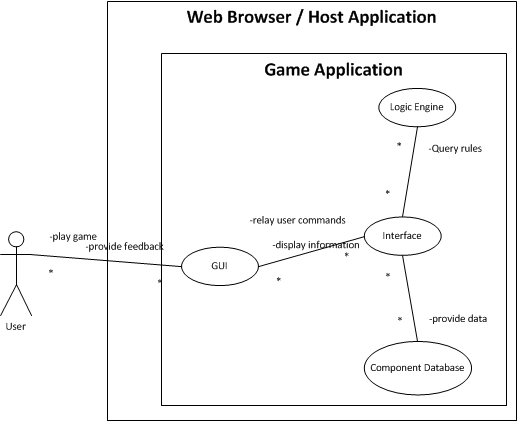
\includegraphics[width=5in]{Resources//Use Case Diagram.png}
\caption{A use-case diagram of the interactions between the sub programs.}
\label{fig:UseCaseDiagram}
\end{figure}

\subsection{Technical Overview\textcolor{red}{[FROM PRESENTATION]}}
\label{sec:Methodology:TechnicalOverview}
\subsubsection{The Component Database\textcolor{red}[FROM PRESENTATION]}
\label{sec:Methodology:TechnicalOverview:TheComponentDatabase}
This is a repository of all elements that can feasibly have an affect 
on the operation of the data centre. Examples include:

\begin{itemize}
\item Cooling systems
\item CPUs
\item Data traffic management algorithms
\item Operating times
\item Average ambient temperatures
\end{itemize}

For each of these, attributes are included, such as power
Consumption (which would be added to the overall power
consumption for the whole data-centre), purchasing cost, ideal operating 
temperature etc.

The Component Database is intended to be extensible, so that 
new technologies can be added As they become available.

Initially, an object oriented approach to the development of the database was taken
The justification of this approch is as follows:

\begin{itemize}

\item Generic classes can be used, which can be defined as being specific variations
 dependant on input parameters An example of this could be the considered to be the various
types of air conditioning system defined in section \ref{sec:ACriticalReviewOfReleventScientificAndEngineeringLiturature:StudiesIntoTheEnvironmentalEffectsAndEnergyEffiencyOfDataCenters:TheDifferentTypesOfAirConditioningEquipmentForITEnvironments}
\cite{TonyEvansTheDifferentTypesOfAirConditioningEquipmentForITEnvironmentsWhitePaper};

\item A switch-case construct could be used to define parameters supplied to an ``air conditioning system"
object at its construction, such as the devices spacial footprint, location within the room and a number 
used to define whether it is an air cooled system, a glycol cooled system, or another.

\end{itemize}

\subsubsection{Isolated testing of the Component Database}

\subsubsection{The Logic Engine\textcolor{red}{[FROM PRESENTATION]}}
\label{sec:Methodology:TechnicalOverview:TheLogicEngine}
It Will be written as a knowledge base, prototyped in a logical programming language such as Prolog or Simulink, before being written in a way that it can be used by the program interface.

Queries will consist of an entity in the Component Database being checked against the list of predicates in the Logic Engine's knowledge base. 

For example, if the user chooses a component, $A$, that has a maximum operating temperature, $T_{max}$, and then the user tries to add another component, $B$ which will raise the ambient temperature, $T_{amb}$ of the data centre above $T{max}$ , then the logic engine will prevent the Program Interface from allowing the user to add $B$.

%\begin{equation}
%\begin{split}
%&P_1 \models A \Rightarrow T_{max} \\
%&P_2 \models B \Rightarrow T_{amb} > T_{max} \\
%&C \models A \and \neg B \Rightarrow T_{amb} < %T_{max} \\
%\end{split}
%\end{equation}

\begin{equation}
\begin{split}
&P_1 \equiv A \Rightarrow T_{max} \\
&P_2 \equiv B \Rightarrow T_{amb} > T_{max} \\
&C \equiv A \land \neg B \Rightarrow T_{amb} < T_{max}
\end{split}
\end{equation}


The testing phase of this element will consist of querying a series of predicates in the knowledge base against dummy data. Once the Logic Engine works to a satisfactory extent, it will be integrated into the Testing Interface and tested against data in the Component Database.

The Logic Engine is intended to be extensible, so that if new principles are discovered that apply, they can be included.

\subsubsection{Isolated testing of the Logic Engine}

\subsubsection{The Program Interface\textcolor{red}{[FROM PRESENTATION]}}
\label{sec:Methodology:TechnicalOverview:TheProgramInterface}
This serves as the interface allowing the user to communicate with 
the program via the GUI, and for the program to query information on 
user selected components
against the logic engine.

It's development life-cycle will be in two stages:

\begin{enumerate}

\item The aforementioned “Testing Interface” will be developed in order to test the compatibility 
of the Component Database and the Logic Engine. As a test program, its input and output 
will primarily be through the command line.

\item The Testing interface will be further developed into the Program Interface by adding the
capacity for it to relay information between the other sub programs and the GUI.

\end{enumerate} 

The Program Interface will be written in JavaScript, allowing integration into a web page coded in HTML5 and CSS.

\subsubsection{Isolated testing of the Program Interface}

\subsubsection{The GUI\textcolor{red}{[FROM PRESENTATION]}}
\label{sec:Methodology:TechnicalOverview:TheGUI}
The GUI will be programmed to communicate with the program interface on the programming interface's terms. This allows multiple developments of the GUI, testing whether 2D or 3D GUIs work best with the game.

\begin{figure}[H]
\centering
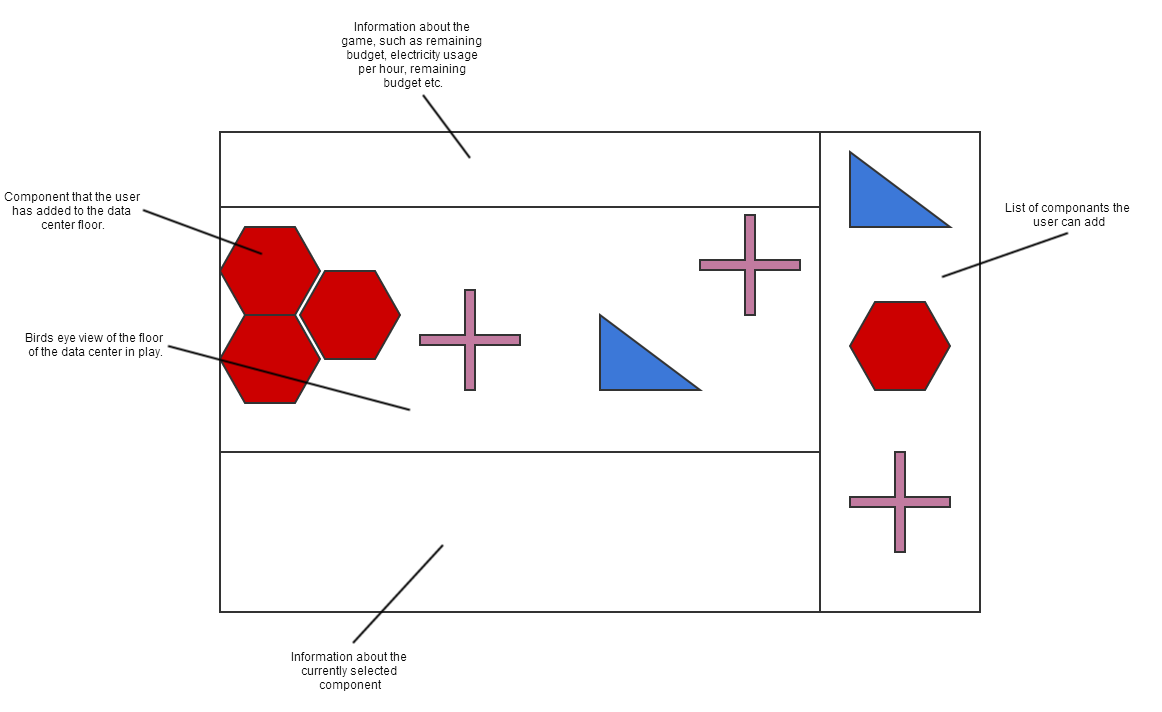
\includegraphics[width=7.25in]{Resources//GUI Mock up.png}
\caption{A mock up example of a potential GUI design, showing a top-down view of the \gls{data centre} floor, allowing users to place components from a list on the right hand side of the screen, with information about the component in the bottom pane, and general game information in the top pane.}
\label{fig:GUIMockUp}
\end{figure}

\subsubsection{Test Cycle One}
\label{sec:DevelopmentOfTheComponentDatabaseAndTheLogicEngineApplicationComponents:TestingOfTheComponentDatabaseAndTheLogicEngineViaTheTestInterface:TestCycleOne}

The first issue found was that...

This was corrected by performing the following actions:
\begin{itemize}
\item
\item
\item
\end{itemize}

The second issue found was that...

This was corrected by performing the following actions:
\begin{itemize}
\item
\item
\item
\end{itemize}

\section{Development of an Interface between the Component-Database and the Logic-Engine, and Development of a GUI}
\label{sec:DevelopmentOfAnInterfaceBetweenTheComponentDatabaseAndTheLogicEngineAndDevelopmentOfAGUI}

\subsection{Interface Development}
\label{sec:DevelopmentOfAnInterfaceBetweenTheComponentDatabaseAndTheLogicEngineAndDevelopmentOfAGUI:InterfaceDevelopment}
\textcolor{red}{The interface will be developed from the Test-Interface (section \ref{sec:DevelopmentOfTheComponentDatabaseAndTheLogicEngineApplicationComponents:TheTestInterface}). As such, this section may become obsolete and be removed.}

\subsection{The GUI}
\label{sec:DevelopmentOfAnInterfaceBetweenTheComponentDatabaseAndTheLogicEngineAndDevelopmentOfAGUI:TheGUI}
\textcolor{red}{Chronicling of the development of the GUI}

\subsection{Integration}
\label{sec:DevelopmentOfAnInterfaceBetweenTheComponentDatabaseAndTheLogicEngineAndDevelopmentOfAGUI:Integration}
\textcolor{red}{Integration of the all of the software components and the GUI together into a working program.}

\fi